\section{Aufbau}
\label{sec:Aufbau}

\begin{figure}
 \centering
 \caption{Eine schematische Darstellung des Messaufbaus \cite{V702}}
 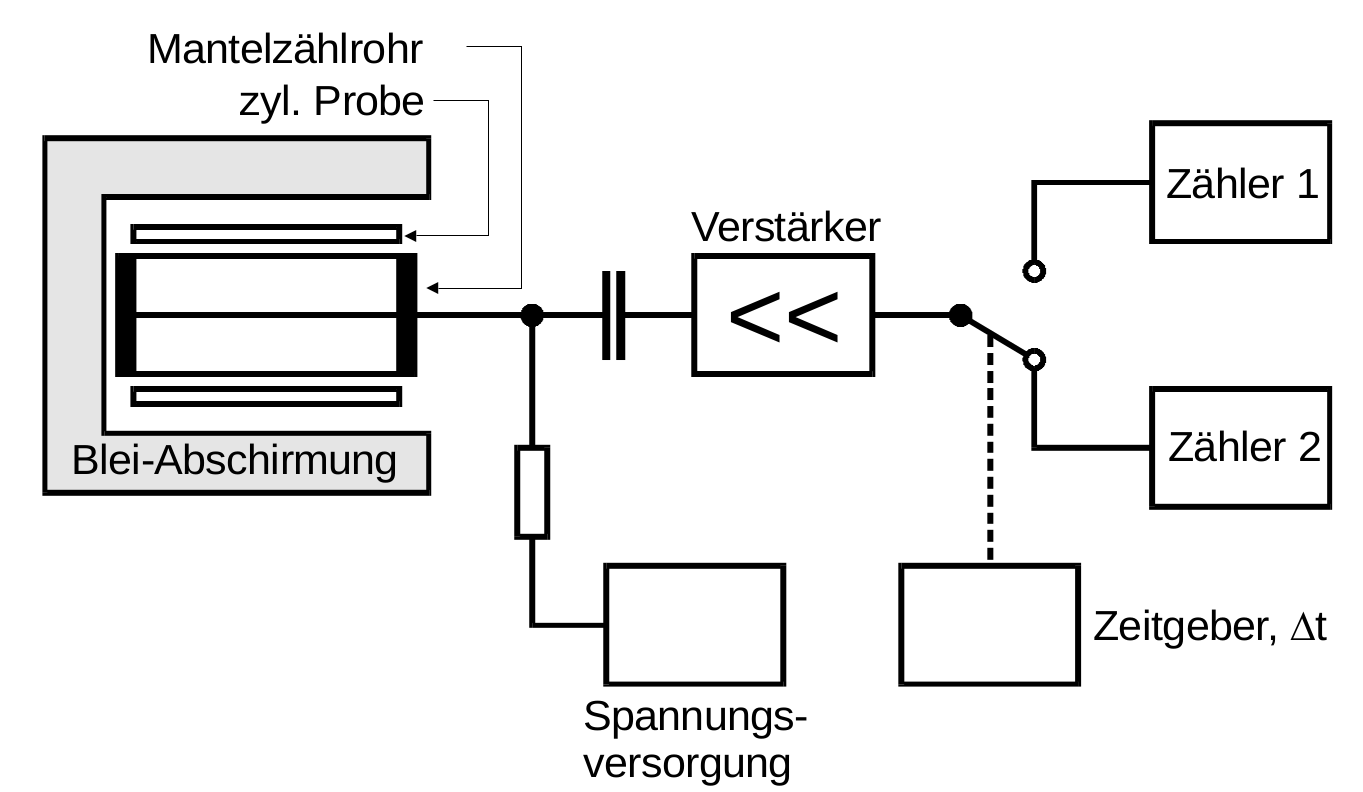
\includegraphics[width=\linewidth-70pt,height=\textheight-70pt,keepaspectratio]{content/aufbau.png}
 \label{fig:aufbau}
\end{figure}

\begin{figure}
 \centering
 \caption{Eine schematische Darstellung der Isotopenanreicherungbehälters \cite{V702}}
 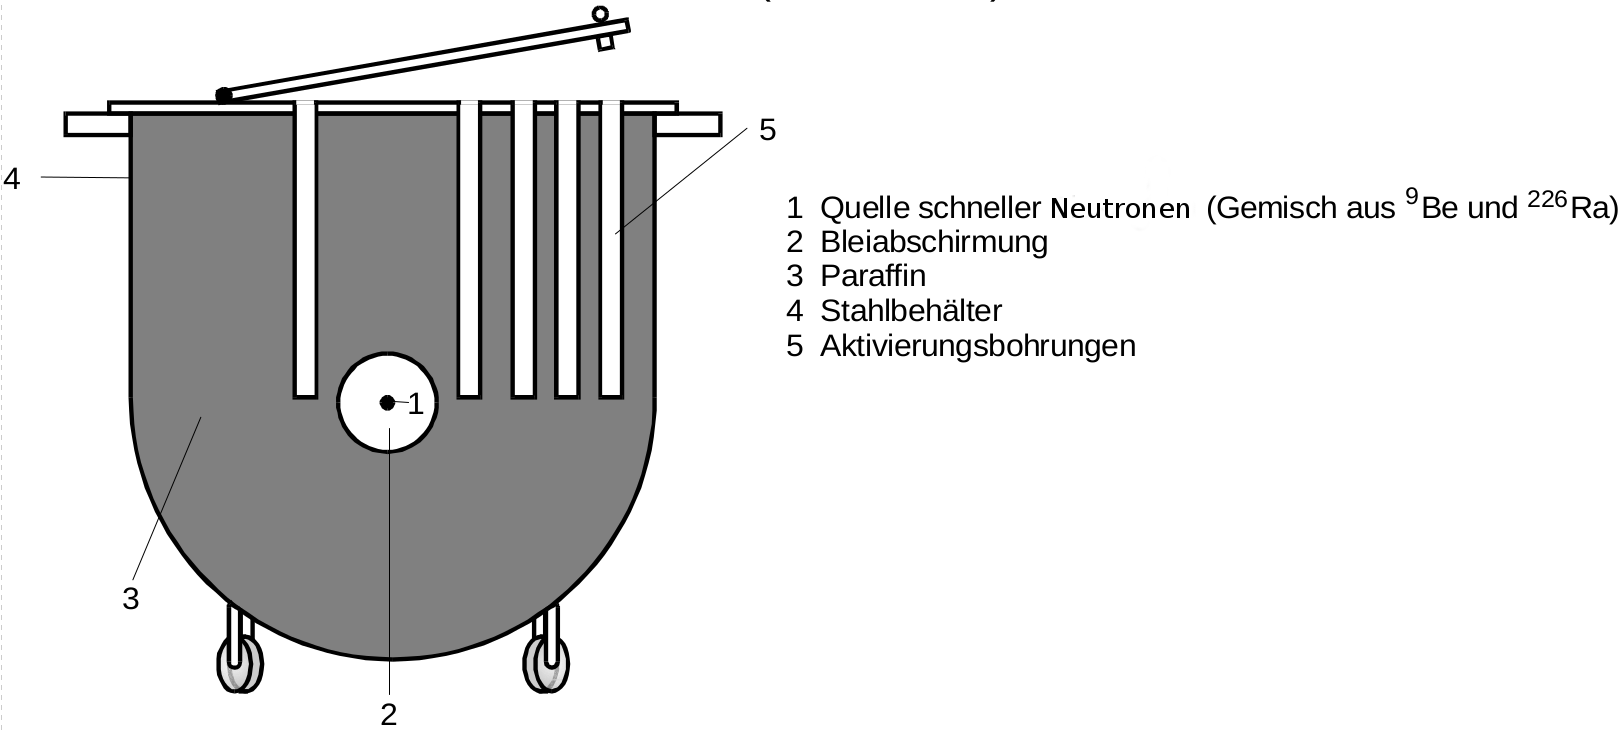
\includegraphics[width=\linewidth-70pt,height=\textheight-70pt,keepaspectratio]{content/kochtopf.png}
 \label{fig:topf}
\end{figure}


Der Messaufbau besteht im Kern aus einem radioaktiven Isotop und einem
 Geiger-Müller-Zählrohr, welches die auftretenden Betateilchen registriert. Dieses besteht aus einer mit Argon gefüllten Röhre. Trifft nun ein Betateilchen oder ein Gammat
 quant auf das Argon, wird dieses ionisiert und sorgt aufgrund einer hohen anliegenden Spannung für eine Elektronenlavine. Die Spannung kann anschließend ohne einen Verstärker gemessen werden. Die Messzeit kann am Auslesegerät der Trefferzahl eingestellt werden. Nach einem Durchlauf wird auf ein zweites Zählwerk gewechselt, sodass die aktuellen Ergebnisse notiert werden können. Zum Schutz vor radioaktiver Strahlung ist der Messaufbau zudem mit einer Bleiverkleidung versehen. Um die benötigten radioaktiven Isotope zu erzeugen, werden stabile Kerne mit Alphastrahlung in einem Behälter nach Abb. \ref{fig:topf} beschossen. Um die Ausbeute zu maximieren durchläuft die Alpha-Strahlung zunächst jedoch eine bremsende Paraffinschicht.
